\documentclass[12pt, letterpaper, twoside]{article}
\usepackage[utf8]{inputenc}%codification of the document

\usepackage{comment}
\usepackage{graphicx}
\usepackage{listings}

\graphicspath{ {.} }

\title{GNU Plot and Diversity in CSE at Notre Dame}
\author{Shane Ryan \thanks{funded by the ShareLaTeX team}}
\date{February 14 2017}

%Here begins the body of the document
\begin{document}

\begin{titlepage}
\maketitle
\end{titlepage}


{\centering\large Overview\par}

This reading assignment explored handling and creating reports based on data in Linux.  I used a Linux shell script to process the data and create a plot.  This helped me better interpret the interesting skew of diversity in the CSE department here. The main takeaway is that computer science is still not a diverse major, though it is improving, and that the Linux command line can be a powerful tool for creating visual representations of data. \par


{\centering\large Methodology\par}


Ultimately I used curl to retrieve the data, cut to select the appropriate columns based on the year and desired information, sort to order the list, and grep to print out the number of matches.  This output was given to gnuplot via a makefile in order to create a graphical representation of the data.\par

In order to print out each year's distribution on a new line, I setup a for loop that stepped through the years provided:


\begin{lstlisting}
for year in $(seq 2013 2019); do                                                                                 
    echo $year $(count_gender $year F) $(count_gender $year M)
done                
\end{lstlisting}

Then, to select the current year's data at each loop iteration, I setup a simple algebraic expression to pick the correct column:

\begin{lstlisting}
column=$(( (($1 - 2012)*2)-1 ))
\end{lstlisting}

Now that we know the column of data needed for the selected year, we can cat all the data into cut (specifying comma as the delimiter) to select that data, use sed to remove blank lines, sort the output, and print the number of matches to our desired attribute using grep:

\begin{lstlisting}
cat demographics.csv | cut -d , -f $column \
| sed '/^$/d' | sort | grep -ce "$2"
\end{lstlisting}

The same approach was used for manipulating the data for ethnicity.  Now a makefile is called to gather the output of the above data processing and send it to gnuplot to generate visual representations.\par

\newpage

{\centering\large Analysis\par}

The following are tables and charts generated from the given data:

\centering


\begin{tabular}{l*{6}{c}r}
              & 2013 & 2014 & 2015 & 2016 & 2017  & 2018 & 2019 \\
\hline
Caucasian         & 43 & 43 & 47 & 53 & 60 & 91 & 92  \\
Asian             & 7 & 5 & 4 & 2 &  1 & 1 &  0  \\
Hispanic          & 7 & 4 & 10 & 9 &  3 & 12 &  10  \\
African          & 3 & 2 & 4 & 1 &  5 & 3 &  3  \\
Native              & 1 & 1 & 1 & 7 &  5 & 4 &  15  \\
Multiple          & 2 & 1 & 1 & 0 &  6 & 8 &  14  \\
Undeclared          & 0 & 0 & 2 & 0 &  0 & 0 &  0  \\
\end{tabular}



\begin{tabular}{ |l|l|l }
  \hline
  \multicolumn{2}{|c|}{Gender Distribution} \\
  \hline
  2013 & M: 49 F: 14  \\
  2014 & M: 44 F: 12 \\
  2015 & M: 58 F: 16 \\
  2016 & M: 60 F: 19 \\
  2017 & M: 65 F: 26 \\
  2018 & M: 90 F: 36 \\
  2019 & M: 97 F: 51 \\

  \hline
\end{tabular}

Clearly the CSE department is predominately white and male.  I am in the
computer ethics course this is related to and the topic has been discussed in
many ways.  Hopefully the trend of diversity in STEM continues to grow and we
obtain a more balanced distribution in the near future.

I feel that although this distribution is skewed, the department creates a
welcoming environment for all those willing to participate.  This is an
outsiders view because I am an Electrical Engineering major.


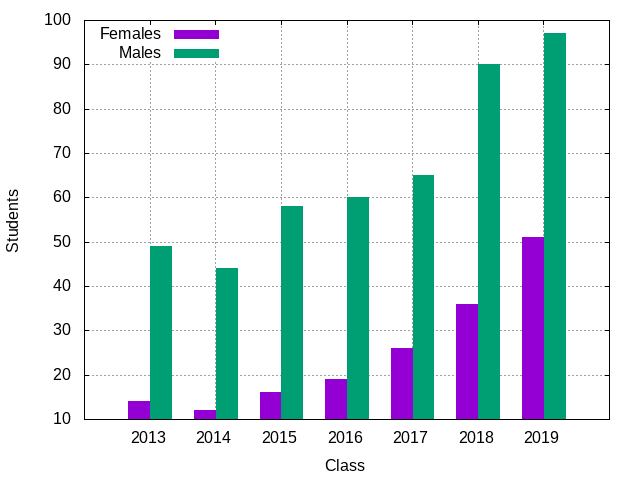
\includegraphics{gender}
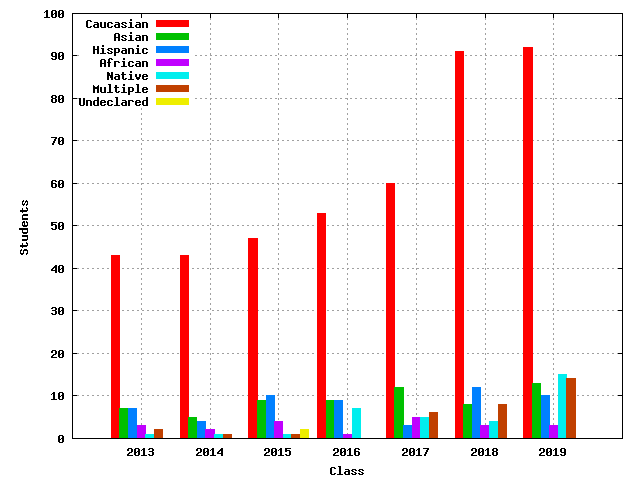
\includegraphics{ethnic}









\begin{comment}
This text won't show up in the compiled pdf
this is just a multi-line comment. Useful
to, for instance, comment out slow-rendering
while working on the draft.
\end{comment}

\end{document}

